\EXERCISE
روش مرتب‌سازی ادغامی
\lr{(Merge Sort)}
: یک روش مرتب‌سازی مبتنی بر مقایسه‌ی عناصر با استفاده از روش تقسیم و غلبه است. این روش از مراحل بازگشتی زیر تشکیل یافته است:
\\
۱- آرایه را به دو زیرآرایه با اندازه‌ی تقریبا یکسان تقسیم کن.
\\
۲- دو زیرآرایه را به دو روش مرتب‌سازی ادغامی مرتب کن.
\\
۳- دو زیرآرایه‌ی مرتب‌شده را ادغام کن.
\begin{center}
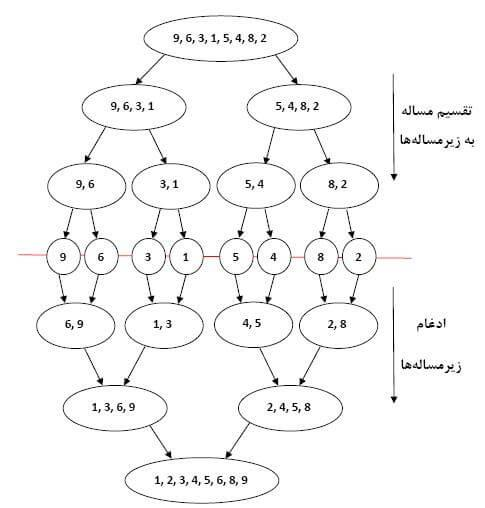
\includegraphics[scale=0.5]{./7.png}
\end{center}
فرض کنید در الگوریتم مرتب‌سازی ادغامی، هزینه‌زمانی لازم برای ادغام دو آرایه، هر کدام به طول
$k$
برابر
$2kt + 1$
باشد که در آن
$t$
واحد زمانی وابسته به پردازنده است (ثابت فرض شود).
$2^m$
عدد نامرتب را در نظر بگیرید که برای مرتب شدن به روش مذکور در اختیار ما قرار گرفته‌اند. اگر داده‌ها را در هر تقسیم دقیقا به دو قسمت مساوی تقسیم کنیم:
\begin{enumerate}
\item
رابطه‌ی بازگشتی برای محاسبه‌ی زمان اجرای الگوریتم را به‌دست آورید (برای مرحله‌ای که دو آرایه به طول
$L$
در حال ادغامند، زمان اجرای آن را 
$T(L)$
بنامید.)
\item
با استفاده از رابطه‌ای که به‌دست آوردید، زمان اجرای برنامه را بر حسب
$m$
و
$t$
به‌دست آورید.
\item
با توجه به پاسخ قسمت (ب)، مرتبه‌ی زمانی الگوریتم را بر حسب
$n$
که
$n = 2^m$
باشد، بیان کنید.

\end{enumerate}
نکته) از زمان صرف شده برای تقسیم کردن آرایه صرف نظر کنید و محاسبات را از اولین گام اقدام آغاز کنید.
\\
راهنمایی) پاسخ قسمت (آ) باید به شکل
$T(L) = f(T(g(L)))$
باشد که در آن
$g$
و
$f$
دو تابع هستند.
\\
نکته) در قسمت‌های (آ) و (ج) فقط پاسخ نهایی اهمیت دارد و بررسی می‌شود.